\subsubsection{Metadata}
\label{sec:view_metadata}

\paragraph{}
The metadata page provides users with the option to assign metadata information (levels of factors, values of continuous variables) to the experimental outcomes. Experimental outcomes are determined by the data parser and held in the database. If no experimental outcomes are defined for an experiment then the metadata functions are unavailable to the user. The main page is split into three main sections as shown in figure \ref{fig:metadata_page_structure}. The first section lists the available experimental outcomes as a series of boxes into which levels of factors or continuous variables may be dragged and dropped (acheived using scriptaculous.js dragables and dropables). The next section lists the available factors and continuous variables for this experiment, which can be dragged into the outcome boxes. Once assiged to an outcome, a piece of metadata can be deleted again using the delete link next to its name in the outcome box. This will only remove the variable from the outcome, variables can be removed from the experiment or deleted from the database completely (assuming they are owned by the current user) using the links in the factors and cont\_vars section of the page. Newly created variables are automatically added to the current experiment. Users may also select from pre-existing variables and add these to the current experiment.


\begin{figure}[h]
\centering
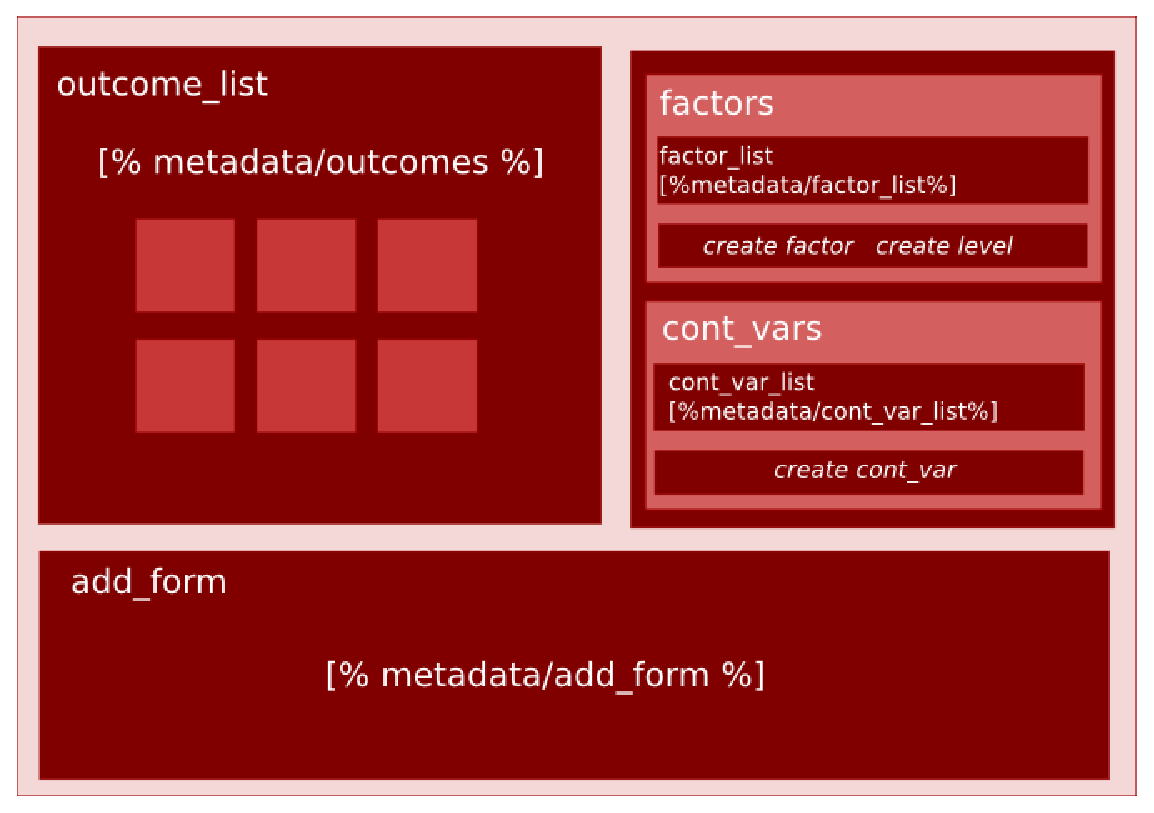
\includegraphics[scale=0.6]{../rome/docs/images/metadata_page_structure}
\caption{Structure of the Metadata Page}\label{fig:metadata_page_structure}
\end{figure}



\begin{figure}[h]
\centering
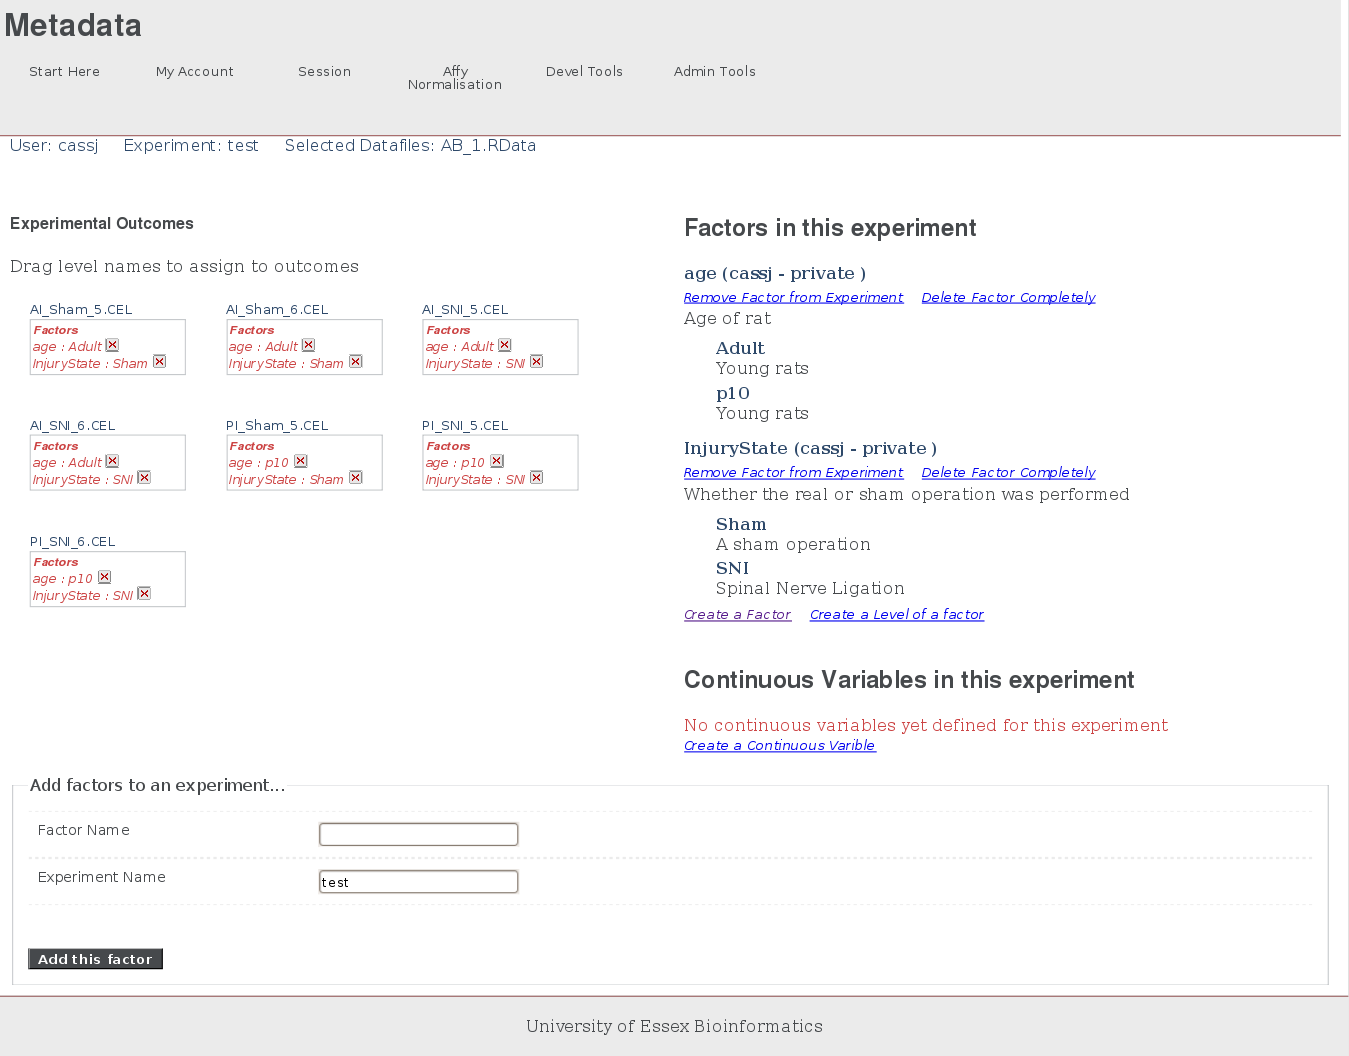
\includegraphics[scale=0.45, angle=90]{../rome/docs/images/screenshots/metadata2}
\caption{The Metadata Page}\label{fig:metadata_view}
\end{figure}

\clearpage